\documentclass[12pt]{article}
\usepackage{../thesis_style}

\title{Chapter 3: Ellipticity and Microlocalisation}
\date{}

\begin{document}
\maketitle

Having defined and developed the calculus of pseudodifferential operators, we now turn to matter concerning solving (\textit{pseudo})differential equations. Typically, we have equation of the form
\begin{align}
Au = f, \quad A \in \Psi^{m}_{\infty}(\R^n), \, u \in \sch'(\R^n), f \in H^s(\R^n). \label{eq: example diff eq}
\end{align}
The goal is to study how regularity and singularity of $Au$ (which is given as $f$), affects that of the solution, $u$, if it exist. 

\section{Pseudodifferential operators are pseudolocal}
We shall show two results pertaining to the singular support of pseudodifferential operators. The first is that the singular support of any pseudodifferential operator  is contained within the diagonal. This is commonly stated as : ``pseudodifferential operators are smooth away from the diagonal, $x = y$". The second result is the pseudolocality result that says that action pseudodifferential operator do not increase singular support of distributions. In terms of differential equation (\ref{eq: example diff eq}), we can say that the solution $u$ is singular at all the points where $f$ is singular. 

\subsection{Support and singular support} 
First, we need the definition of support and singular support of both operators and distributions. Roughly, the support of a distribution in $\R^n$ consist of points $x \in \R^n$ where the distribution is non-zero after any smooth cut-offs near $x$. 
\begin{fdefinition}
    The \textbf{support of a tempered distribution} $u \in \sch'(\R^n)$ is given by the set
    \[
    \supp(u) = \set{x \in \R^n \wh \exists \chi \in \sch(\R^n), \chi(x) \neq 0, \chi u = 0}^c. 
    \]
    \\
    
\end{fdefinition}
\hfill \\
And the singular support of a distribution is the set of points where the distribution fails to behave like an element of $\sch(\R^n)$, i.e. it is either not $C^\infty$ or does not have rapid decay. 
\begin{fdefinition}
    The \textbf{singular support of a tempered distribution} $ u \in \sch'(\R^n)$ is given by the set 
    \[
    \mathrm{sing supp}(u) = \set{x \in \R^n \wh \exists \phi \in S(R^n), \phi(x) \neq 0, \phi(u) \in \sch(\R^n)}^c
    \]
\end{fdefinition}
\begin{rem} \hfill 
    \begin{itemize}
        \item     Note that if the singular support of a tempered distribution is empty, it is then an element of $C^\infty(\R^n)$.     
        \item  Both the supports or singular supports are presented above as complement of open sets, therefore they are closed. \\
        
    \end{itemize}

\end{rem}

The support of an operator is given by the support of its Schwartz kernel. 

\begin{fdefinition}
    The \textbf{support of a continuous linear operator} $A: S(R^n) \to \sch'(\R^n)$ is given by 
    \[
    \supp(A) = \supp(K_A) \subset \R^n \times \R^n
    \]
    where $K_A \in \sch'(\R^n \times \R^n)$ is the Schwartz kernel of $A$. 
\end{fdefinition}


%We have the following result relating the support of a smooth function after the action of a continuous linear operator. 
%\begin{fprop}[Calculus of support]
%    Let $A: \sch(\R^n) \to \sch(\R^n)$ be a continuous linear operator and $\phi \in C^\infty_c(\R^n)$, then
%    \[
%    \supp(A \phi) \subset \supp(A) \circ \supp(\phi) := \set{x \in \R^n \wh \exists y \in \supp(\phi), (x, y) \in \supp(A) }. 
%    \]
%\end{fprop}
%\begin{proof}
%    We shall show the contrapositive statement:
%    \[
%    x \not \in \supp(A) \circ \supp(\phi) \implies x \not \in \supp(A \phi). 
%    \]
%    Suppose $x \not \in \supp(A) \circ \supp(\phi)$. Observe that 
%    \[
%    \supp(A) \circ \supp(\phi) = \pi_x(\pi_y^{-1}(\supp(\phi)) \cap \supp(A))
%    \]
%    where $\pi_{x, y} : \R^2 \to \R$ are the projection map to the respective coordinates. Since $\supp(A)$ is closed and $\supp(\phi)$ is compact, we have that $\supp(A) \circ \supp(\phi)$ is closed and thus $x$ belongs to an open set. We can therefore choose a smooth cutt-off function $\chi \in C^\infty_c(\R^n)$ supported at $x$ ($\chi(x) \neq 0$) but away from $\supp(A) \circ \supp(\phi)$. Thus, 
%    \[
%    \supp(A) \cap (\supp(\chi) \times \supp(\phi)) = \emptyset
%    \]
%    and hence $\chi(x) K_A(x, y) \phi(y) = 0 \implies \chi A \phi = 0$, as required. 
%\end{proof}
%
%
%

Now, we are ready to show that pseudodifferential operators are smooth away from the diagonal. 

\begin{fprop}
    Let $A \in \Psi^m_\infty(\R^n)$ for some $m \in \R$, then
    \[
    \mathrm{sing supp}(A) \subset \set{(x, y) \in \R^{2n} \wh x = y}. 
    \]
\end{fprop}
\begin{proof}
    Using lemma (\ref{lemma: density of residual symbols}), it suffices to prove this theorem for elements of $\Psi^{-\infty}_\infty(\R^n)$ and then extend by continuity to all orders. \\
    
    Let $A \in \Psi^{-\infty}_\infty(\R^n)$ with symbol $a \in S^{-\infty}_\infty(\R^{2n}; \R^n)$. Its singular support is given by the singular support of the kernel. Since all derivatives of $a$ are $O(\sym[\xi]^{-\infty})$, the oscillatory integral below representing the kernel is absolutely convergent  and, using integration by parts, we get
    \begin{align*}
        I(a) 
        & = \frac{1}{(2\pi)^n} \int e^{i(x - y) \cdot \xi} a(x, y, \xi) \d[\xi] \\
        & = \frac{1}{(2\pi)^n}  \int \frac{1}{(x - y)^\alpha} (-D^\alpha_\xi) \brac{e^{i(x - y) \cdot \xi} }a(x, y, \xi) \d[\xi] \\
        & = \frac{1}{(x - y)^\alpha} \frac{1}{(2\pi)^n} \int e^{i(x - y) \cdot \xi} (-D^\alpha_\xi) a(x, y, \xi) \d[\xi] \\
        & = \frac{1}{(x - y)^\alpha} I((-D^\alpha_\xi)a)
    \end{align*}
    which is true for all multi-index $\alpha$ of any order. Since all $x, y$-derivatives of $a$ are uniformly bounded by $\sym[\xi]^{-N}$ for any $N \in \N$, we can differentiate under the integral sign to get the equation
    \begin{align*}
        D^\beta_x D^\gamma_y (x - y)^\alpha I(a) 
        & = \frac{1}{(2\pi)^n} \int D^\beta_x D^\gamma_y e^{i(x - y) \cdot \xi} (-D^\alpha_\xi) a(x, y, \xi) \d[\xi] \\
        & = \frac{1}{(2\pi)^n} \int (-1)^{\abs{\beta}}\xi^{\beta + \gamma}e^{i(x - y) \cdot \xi} (-D^\alpha_\xi) a(x, y, \xi) \d[\xi] \\
    \end{align*}
    where the last integral gives a smooth function, thus showing that $(x - y)^\alpha I(a)$ is smooth for all $\alpha$, and hence $I(a)$ is smooth away from $x = y$. \\
    \\
%    Now, for a general $A \in \Psi^m_\infty(\R^n)$, $m \in \R$, we shall use the  density of $S^{-\infty}_\infty(\R^{2n}; \R^n) \subset S^{m}_\infty(\R^{2n}; \R^n)$ and that $I$ extends by continuity to a map $I : S^{m}_\infty(\R^{2n}; \R^n) \to \sch'(\R^{2n})$ in the topology $S^{m + \epsilon}_\infty(\R^{2n}; \R^n)$ for any $\epsilon > 0$  \ref{}. 
%    
%    
\end{proof}


\begin{fprop}
    Let $A \in \Psi^m_\infty(\R^n)$ for some $m \in \R$ and $u \in \sch'(\R^n)$ be compactly supported tempered distribution, then 
    \begin{align*}
        \mathrm{sing supp}(A u) \subset \mathrm{sing supp }(u). 
    \end{align*}
    We call operators that satisfies the above property \textit{pseudolocal} operators.
\end{fprop}
\begin{proof}
    Again we shall prove the contrapositive statement: 
    \[
    x \not \in \mathrm{sing supp}(u) \implies x \not \in \mathrm{sing supp}(Au)
    \]
    Let $u \in \sch'(\R^n)$ be compactly supported and $x_0 \not \in \mathrm{sing supp}(u)$.  We can choose $\chi \in \sch(\R^n)$, (normalised) so that $\chi \equiv 1$ in a neighbourhood of $x_0$ and that $\chi u \in \sch(\R^n)$. Observe that 
    \begin{align*}
        Au = A(\chi u + (1 - \chi)u) = A(\chi u) + A(1 - \chi)u. 
    \end{align*}
    Since $\chi u \in \sch(\R^n) \implies A\chi u \in \sch(\R^n)$ (proposition \ref{prop : schwartz to schwartz}), we have that 
    \begin{align*}
        \mathrm{singsupp}(Au) = \mathrm{singsupp}(A(1 - \chi)u). 
    \end{align*}
    Furthermore, we know that $x_0 \not \in \supp((1 - \chi)u)$. 
    Now, we shall further cut-off near $x_0$ by choosing a $\phi \in \sch(\R^n)$ compactly supported  away from $\supp(1 - \chi)$ and $\phi \equiv 1$ near $x_0$, i.e. 
    \[
    \supp(1 - \chi) \cap \supp \phi = \emptyset. 
    \]
    We now have an operator $\phi A(1 - \chi) $ with kernel
    \[
    \phi(x) K_A(x, y) ( 1 - \phi(y))
    \]
    that vanishes (in particular smooth) on the diagonal. Since we have shown that the singular support of a pseudodifferential operator have to be contained in the diagonal, we conclude that $\phi A(1 - \chi)$ is a smoothing operator, and thus $\phi A (1 - \chi) u \in C^\infty(\R^n)$ as required. 
    
\end{proof}


\section{Global ellipticity} 
There is a subset of operators for which we can conclude much more than just pseudolocality, namely the set of operators that are \textit{elliptic}. These are elements of the algebra $\Psi^{\infty}_{\infty}$ that are invertible up to additive elements in $\Psi^{-\infty}_{\infty}(\R^n)$. 

\begin{fdefinition}
    A pseudodifferential operator $A \in \Psi^{m}_{\infty}(\R^n)$ is elliptic if there exist $B \in \Psi^{-m}_{\infty}(\R^n)$ such that 
    \begin{align*}
    A \circ B - 1 \in \Psi^{-\infty}_{\infty}(\R^n). 
    \end{align*}
    The approximate inverse $B$ is known as the (global) \textbf{elliptic parametrix} of $A$. 
\end{fdefinition}

A canonical example of elliptic differential operator is the Helmholtz operator 
\begin{align*}
1  + \Delta = 1 - \sum_{j = 1}^ n \p_{x_j}^2 \in \Psi^{2}_{\infty}(\R^n)
\end{align*}
which has explicitly invertible left reduced symbol $\abs{\xi}^2 + 1$ and principal symbol $\abs{\xi}^2$. Using the calculus of symbols, we know that $(1 + \Delta)^{-1}$ is simply the pseudodifferential operator that acts as 
\begin{align*}
(1 + \Delta)^{-1} u(x) = I\brac{\frac{1}{1 + \abs{\xi}^2} } u(x) = \frac{1}{(2\pi)^n} \int e^{i(x - y) \cdot \xi} \frac{1}{1 + \abs{\xi}^2} u(y) \d[y] \d[\xi]
\end{align*}
We will find out later that ellipticity is in fact a property of the \textit{principal symbol} only. Thus, the Laplacian $\Delta$ which has the same principal symbol $\abs{\xi}^2$ is also elliptic as expected from traditional theory on differential operators. 


\todo{motivation for elliptic symbols} 
\subsection{Elliptic symbols}
\begin{fdefinition}
    Given $p, n \in \N$ and $m \in \R$, an order $m$ symbol $a \in S^m_\infty(\R^p; \R^n)$ is (globally) \textbf{elliptic} if there exist $\epsilon \in \R_{>0}$ such that 
    \[
    \inf_{\abs{\xi} \geq 1/\epsilon} \abs{a(x, \xi)} \geq \epsilon \sym[\xi]^m. 
    \]
\end{fdefinition}

The importance of elliptic symbol is that they are invertible modulo $S^{-\infty}_\infty(\R^p; \R^n)$ as shown in the next lemma. 

\begin{flemma}
    Let $p, n \in \N$, $m \in \R$ be given and let $a \in S^m_\infty(\R^p; \R^n)$ be an elliptic symbol of order $m$. Then there exist a symbol $b \in S^{-m}_\infty(\R^p; \R^n)$ such that 
    \[
    a \cdot b - 1 \in S^{-\infty}_\infty(\R^p; \R^n). 
    \]
\end{flemma}
\begin{proof}
    We shall follow the general strategy of inverting the symbol outside of a compact set. Let $\phi \in C^\infty_c(\R^n)$ be a smooth cut off function, i.e $0 \leq \phi \leq 1$ and $ \phi(\xi) = 1$ for $\abs{\xi} < 1$ and $\phi(\xi) = 0 $ for $\abs{\xi} > 2$. \\
    
    Let $a \in S^{m}_\infty(\Omega; \R^n)$ be an elliptic symbol, that is, for any fixed $\epsilon \in \R_{> 0}$, we have 
    \[
    \abs{a(x, \xi)} \geq \epsilon \sym[\xi]^m
    \]
    for any $\abs{\xi} \geq 1/\epsilon$. Thus, we can define 
    \begin{align*}
    b(x, \xi) = 
    \begin{cases}
    \frac{1 - \phi( \epsilon \xi /2)}{a(x, \xi)} & \abs{\xi} \geq 1/ \epsilon \\
    0 & \abs{\xi} < 1 / \epsilon. 
    \end{cases}
    \end{align*}
    It remains to check: 
    \begin{description}
        \item[$b$ is well-defined and smooth. ] \hfill \\
        We note that $\abs{a(x, \xi)} > 0$ whenever $\abs{\xi} \geq 1/\epsilon$ and therefore $b$ is well defined in that region. For smoothness, we note first that $b$ is smooth in the regions $\abs{\xi} > 1/ \epsilon$ and $\abs{\xi} < 1/\epsilon$. Set $\delta = 1/(2 \epsilon)$. In the region where $1/\epsilon - \delta < \abs{\xi} < 1/\epsilon + \delta$, we have $\abs{\epsilon \xi/ 2} < 1/\epsilon$ and therefore $b(x, \xi) \equiv 0$ in this region and is thus smooth. Since the we have covered $\Omega \times \R^n$ by the three chart domain above, $b$ is smooth by the (smooth) gluing lemma. 
        
        \item[$b$ is a symbol of order $-m$.  ] \hfill \\
        We can prove by induction that in the region $\abs{\xi} \geq 1/ \epsilon$
        \begin{align*}
        D^\alpha_x D^\beta_\xi b = a^{-1 - \abs{\alpha} - \abs{\beta}} G_{\alpha \beta}
        \end{align*}
        for all multi-index $\alpha, \beta$, where $G_{\alpha \beta}$ is a symbol of order $(\abs{\alpha} + \abs{\beta})m  - \abs{\beta}$. Therefore, using the ellipticity estimate for $a$, we get 
        \begin{align*}
        \norm[b]_{k, -m} 
        & = \sup_{(x, \xi) \in \mathrm{Int}(\Omega) \times \R^n} \frac{\abs{D^\alpha_x D^\beta_\xi b(x, \xi)}}{\sym[\xi]^{-m-k}} \\
        &= \sup_{\abs{\xi} \geq 1/\epsilon} \abs{a^{-1 - \abs{\alpha} - \abs{\beta}} G_{\alpha \beta}} \sym[\xi]^{m + k} \\
        &\leq \frac{\norm[G_{\alpha \beta}]_{0, (\abs{\alpha} + \abs{\beta})m - \abs{\beta}}}{\epsilon} \sup_{\abs{\xi} \geq 1/\epsilon^{1 + \abs{\alpha} + \abs{\beta}}} \sym[\xi]^{-m(1 + \abs{\alpha} + \abs{\beta})} \sym[\xi]^{m + k}\\
        & < \infty
        \end{align*}
        as required. 
        
        \item[$b$ is an inverse of $a$ modulo $ S^{-\infty}_\infty(\Omega; \R^n)$. ] \hfill \\
        The main observation is that the set where $b$ fails to be the multiplicative inverse of $a$ is a compact set (in $\xi$) and thus $a \cdot b - 1$ is in fact a compactly supported smooth function of $\xi$ which is a subset of $S^{-\infty}_\infty(\Omega; \R^n)$.  Explicitly, for any $N \in \N$
        \begin{align*}
        \sup_{(x, \xi) \in \mathrm{Int}(\Omega) \times \R^n} \frac{\abs{D^\alpha_x D^\beta_\xi (a\cdot b - 1)} }{\sym[\xi]^{-N}}
        &\leq \sup_{\abs{\xi} \leq 1/ \epsilon} \sym[\xi]^N \abs{D^\alpha_x D^\beta_\xi (\phi(\xi \epsilon / 2))} < \infty.  
        \end{align*}
    \end{description}\end{proof}

\subsection{Elliptic pseudodifferential opertors}
The following theorem characterise globally elliptic pseudodifferential operators. 
\begin{ftheorem}
    Let $A \in \Psi^{m}_{\infty}(\R^n)$ be a pseudodifferential operator. Then, the following are equivalent
    \begin{enumerate}
        \item $A$ is an elliptic pseudodifferential operator.
        
        \item $\sigma_L(A) \in S^{m}_\infty(\R^{n}; \R^n)$ is an elliptic symbol.
                
        \item $\exists b \in S^{- m}_\infty(\R^{n}; \R^n)$, s.t. $\sigma_L(A) \cdot b -1 \in S^{-\infty }_\infty(\R^{n}; \R^n)$. 
        
        \item the principal symbol of $A$ is invertible in the quotient symbol space, i.e. 
        \begin{align*}
        \exists [b] \in S^{m - [1]}_\infty(\R^{n}; \R^n), \quad s.t. \quad \sigma_m(A) \cdot [b] = [1] \in S^{0 - [1]}_\infty(\R^{n}; \R^n)
        \end{align*}
        where $S^{m-[1]}_\infty(\R^{n}; \R^n)$ denotes the quotient space $S^{m}_\infty(\R^{n}; \R^n) / S^{m -1}_\infty(\R^{n}; \R^n)$. 

    \end{enumerate}
\end{ftheorem}
\begin{proof}
    Note that we already have $(2) \iff (3)$ from the previous lemma. We remark that $(1) \implies (4)$ is simply the application of the assuming property of principal symbol under composition on the elliptic parametrix of $A$. For full proof, see \cite{Vasy2015-oo} or \cite{rbm_intro_microlocal}. \todo{reference}
    
\end{proof}


An important characteristic of elliptic pseudodifferential operators is that they are completely regularising. In particular, solutions to $Au = f$ have to be smooth if we know that $f$ is smooth. For instance, solutions to homogeneous equations $Au = 0$ have to be smooth. 

\begin{fprop}
    Let $A \in \Psi^{m}_{\infty}(\R^n)$  be  elliptic. For any $u \in \sch'(\R^n)$, 
    $$Au \in \sch(\R^n) \implies u \in \sch(\R^n). $$ 
\end{fprop}
\begin{proof}
    Let $B \in \Psi^{-m}_{\infty}(\R^n)$ be the elliptic parametrix to $A$ so that $E:= BA - 1 \in \Psi^{-\infty }_{\infty}(\R^n)$. We have
    \begin{align*}
    u = 1 \cdot u = (BA + E)u = BAu + Eu. 
    \end{align*}
    Since $Eu \in \sch(\R^n)$ by proposition (\ref{prop : residual operators are smoothing}), and  we have assumed $Au \in \sch(\R^n)$, we conclude that $u \in \sch(\R^n)$. 
    
\end{proof}

\begin{fprop}
    Let $A \in \Psi^{m}_{\infty}(\R^n)$ be elliptic and $u \in H^{N}(\R^n)$ for some $N \in \R$. Then, for any $s \in \R$
    \begin{align*}
    Au \in H^{s}(\R^n) \implies u \in H^{s + m}(\R^n)
    \end{align*}
    and $u$ satisfies the estimates: $\exists C > 0$
    \begin{align*}
    \norm[u]_{H^{s + m}} \leq C \brac{\norm[Au]_{H^s} + \norm[u]_{H^N}}. 
    \end{align*}
\end{fprop}
\begin{proof}
    Again, let $B \in \Psi^{-m}_{\infty}(\R^n)$ be the elliptic parametrix so that $E := BA - 1 \in \Psi^{-\infty}_{\infty}(\R^n)$. We know that $B : H^{s} \to H^{s + m}$ and  $E : H^N \to H^{s + m}$ are bounded linear map. Using $u = BAu + Eu$, we have
    \begin{align*}
     \norm[u]_{H^{s + m}} \leq \norm[BAu]_{H^{s + m}} + \norm[u]_{H^{s + m}} \leq C \brac{\norm[Au]_{H^s} + \norm[u]_{H^N}}
    \end{align*}
    for some $C > 0$. 
\end{proof}


\section{Microlocalisation}
The principal symbol $\sigma_m$ captures the leading order behaviour of a pseudodifferential operator when the fibre variable $\xi$ is large. In this chapter, however, we will develop further concepts that describes behaviour of a pseudodifferential operator in different \emph{direction} in the phase space, $T^*\R^n$. Of central importance are 
\begin{description}
    \item[Characteristic set] $\Char^m(A) \subset T^*_{x, \xi} \R^n$ of an operator $A \in \Psi^{m}_{\infty}(\R^n)$ describes points in phase space where $A$ is not locally elliptic. This will lead to the notion of microlocal ellipticity. 
    \item[Operator wavefront set] $\WF'(A) \subset T^*_{x, \xi} \R^n$ describes the directions $\xi$ in the fibre of $x$ where $A$ is not ``trivial". 
\end{description}


\subsection{Elliptic set of pseudodifferential operator}
Instead of global ellipticity, we will now define a notion of \textit{ellipticity at a point} in phase space which allow up to define various microlocal contructions that focus on  localised (conically in phase space) behaviour. 

\begin{fdefinition}
    A pseudodifferential operator, $A \in \Psi^m_\infty(\R^n), m \in \R$ is \textbf{elliptic at a point} $(x_0, \xi_0) \in \R^n \times \R^n \setminus \set{0}$ if there exist $\epsilon > 0$ such that its left-reduced symbol satisfies the lower bound
    \[
    \abs{\sigma_L(A)(x, \xi)} \geq \epsilon \sym[\xi]^m
    \]
    in the region
    \[
    \overline{U}_\epsilon = \set{(x, \xi) \in \R^n \times \R^n \setminus \set{0} \wh \abs{x - x_0} \leq \epsilon, \abs{\widehat{\xi} - \widehat{\xi_0}} \leq \epsilon, \abs{\xi} \geq 1/\epsilon}
    \]
    where $\widehat{\xi} = \xi / \abs{\xi}$ denotes the unit vector in the direction of $\xi$ for any non-zero $\xi \in \R^n$. We denote the set of all elliptic points of $A$ as 
    \[
    \Ell^m(A) = \set{(x, \xi) \in \R^n \times \R^n \setminus \set{0} \wh A \text{  is elliptic of order $m$ at } (x, \xi)}
    \]
    and its complement in $\R^n \times \R^n \setminus \set{0}$ as 
    \begin{align*}
        \Char^m(A) 
        &= \Ell^m(A)^c \setminus \set{(x, 0)\wh x \in \R^n} \\
        &= \set{(x, \xi) \in \R^n \times \R^n \setminus \set{0} \wh A \text{  is \textbf{not} elliptic of order $m$ at } (x, \xi)}
    \end{align*}
\end{fdefinition}

\begin{flemma}
    Let $A \in \Psi^m_\infty(\R^n), m \in \R$. 
    \begin{enumerate}
        \item If $\sigma_m(A)(x, \xi)$ is homogeneous of degree $m$ in $\xi$, then 
        \[
        \Ell^m(A) = \set{(x_0, \xi_0) \wh  \xi_0 \neq 0, \sigma_m(A)(x_0, \xi_0) \neq 0}. 
        \]
        \item $\Ell^m(A) $ is open in $\R^n \times \R^n$. 
        \item $\Ell^m(A)$ is conic in $\R^n \times \R^n \setminus \set{0}$, in the sense that 
        \[(x_0, \xi_0) \in \Ell^m(A) \implies (x_0, t \xi_0) \in \Ell^m(A), \forall t \in \R_{>0}.\] 
        \item $\Char^m(A)$ is closed conic. 
        \item if $B \in \Psi^{m'}(\R^n)$, then 
        \[\Char^{m + m'}(A \circ B) = \Char^m(A) \cup \Char^{m'}(B).\]
    \end{enumerate}
\end{flemma}
\begin{proof}
    Let $A \in \Psi^m_\infty(\R^n)$, $m \in \R$ be given. 
    \begin{enumerate}
        \item Suppose the principal symbol $\sigma_m(A)(x, \xi)$ is homogeneous of order $m$ in $\xi$. We need to show that 
        \[
        (x_0, \xi_0) \in \Ell^m(A) \iff \xi_0 \neq 0, \, \sigma_m(A)(x_0, \xi_0) \neq 0. 
        \]
        If $\xi_0 = 0$, $(x_0, \xi_0) \not \in \Ell^m_\infty$ by definition of ellipticity. If $\sigma_m(x_0, \xi_0) = 0$, by homogeneity, we have 
        \[
        \sigma_m(x_0, t \xi_0) = t^m \sigma_m(x_0, \xi_0) = t^m \cdot 0 = 0
        \]
        for all $t \in \R_{> 0}$. By definition of principal symbol, we can write the left symbol of $A$ as 
        \[
        \sigma_L(A) = \sigma_m(A) + a
        \]
        where $a \in S^{m -1}_\infty(\R^n; \R^n)$. Now, observe that for any $\epsilon > 0$, the set 
        \[
        \overline{U}_\epsilon = \set{(x, \xi) \in \R^n \times \R^n \setminus \set{0} \wh \abs{x - x_0} \leq \epsilon, \abs{\widehat{\xi} - \widehat{\xi_0}} \leq \epsilon, \abs{\xi} \geq 1/\epsilon}
        \]
        contains the(open) half-line starting at $\widehat{\xi_0} / \epsilon$, i.e. the set $\set{(x_0, t \xi_0/(\abs{\xi_0}\epsilon)\wh t > 0}$. However, by the symbol estimate of $a$, 
        \begin{align*}
            \abs{\sigma_L(A)\brac{x_0, \frac{t \xi_0}{\abs{\xi_0} \epsilon}}}
            & \leq \brac{\frac{t}{\epsilon \abs{\xi_0}}}^m \abs{\sigma_m(x_0, \xi_0)} + \abs{a\brac{x_0, \frac{t \xi_0}{\abs{\xi_0} \epsilon}}} \\
            & = 0 + \abs{a\brac{x_0, \frac{t \xi_0}{\abs{\xi_0} \epsilon}}} \\
            & \leq C \sym[\frac{t \xi_0}{\abs{\xi_0} \epsilon}]^{m - 1} \\
            & = C\sym[t/\epsilon]^{m - 1}
        \end{align*}
        and therefore 
        \begin{align*}
            \inf_{(x, \xi) \in \overline{U}_\epsilon} \frac{\abs{\sigma_L(A)(x, \xi)}}{\sym[\xi]^m} 
            & \leq \inf_{t > 0}  \frac{\abs{\sigma_L(A)\brac{x_0, \frac{t \xi_0}{\abs{\xi_0} \epsilon}}} }{\sym[t /\epsilon]^m} \\
            & \leq \inf_{t > 0}  \frac{C\sym[t/ \epsilon]^{m - 1} }{\sym[t /\epsilon]^m} \\
            & = C\inf_{t > 0} \sym[t/\epsilon]^{-1}\\
            & = 0
        \end{align*}
        which means that $(x_0, \xi_0) \not \in \Ell^m(A)$. \\
        \\
        Conversely, if $\sigma_m(A)(x_0, \xi_0) \neq 0$, by continuity and homogeneity,  $\sigma_m(A)$, is non-zero in a (closed) conic neighbourhood, i.e. there exist $\epsilon > 0$ such that $\sigma_m(A) \neq 0$ in 
        \begin{align*}
            \overline{U}_\epsilon = \set{(x, \xi) \wh \abs{x - x_0} \leq \epsilon, \abs{\widehat{\xi} - \widehat{\xi_0}}\leq \epsilon, \abs{\xi} \geq 1/ \epsilon}. 
        \end{align*}
        Again, writing the left symbol as a sum of the principal symbol an a lower order term, we observe that in $\overline{U}_\epsilon$, 
        \begin{align*}
            \frac{\abs{\sigma_L(A)(x, \xi)} }{\sym[\xi]^m}
            & \geq \frac{\abs{\abs{\sigma_m(A)(x, \xi)} - \abs{a(x, \xi)}}}{\sym[\xi]^m} \\
            & = \abs{\frac{\abs{\xi}^m}{\sym[\xi]^m} \abs{\sigma_m(A)(x, \widehat{\xi})} - \frac{\abs{a(x, \xi)}}{\sym[\xi]^m}} \\
        \end{align*}
        By the symbol estimate of $a$, the second term is tending to $0$ which the first term is bounded below by $C = \inf_{(x, \xi) \in \overline{U}_\epsilon} \abs{\sigma_m(A)(x, \xi)} > 0$. Therefore, choosing a smaller $\epsilon$ if necessary, we have $\abs{a(x, \xi)} / \sym[\xi]^m < C$ and thus 
        \begin{align*}
            \inf_{(x, \xi) \in \overline{U}_\epsilon} \frac{\abs{\sigma_L(A)(x, \xi)} }{\sym[\xi]^m}
            \geq C' 
            \geq \epsilon. 
        \end{align*}
        and therefore $(x_0, \xi_0) \in \Ell^m(A)$. 
        
        \item We note first that if the principal symbol is homogeneous of degree $m$, the previous result applies and continuity of the principal symbol guarantee that the elliptic set is open (if $\sigma_m(A)$ is non-zero at a point, it is non-zero in an open neighbourhood of the point). \\
        \\
        For the general case, suppose $(x_0, \xi_0) \in \Ell^m(A)$. We therefore have for some $\epsilon > 0$, 
        
        \[
        \abs{\sigma_L(A)(x, \xi)} \geq \epsilon \sym[\xi]^m
        \]
        in the region
        \[
        \overline{U}_\epsilon(x_0, \xi_0) = \set{(x, \xi) \in \R^n \times \R^n \setminus \set{0} \wh \abs{x - x_0} \leq \epsilon, \abs{\widehat{\xi} - \widehat{\xi_0}} \leq \epsilon, \abs{\xi} \geq 1/\epsilon}. 
        \]
        
        It suffice to show that there is an open neighbourhood of $(x_0, \xi_0)$ where $A$ remains elliptic. We can take desired open neighbourhood to be 
        \begin{align*}
            V = \set{(x', \xi') \wh \xi' \neq 0, \, \abs{x' - x_0} < \epsilon/ 2, \, \abs{\widehat{\xi'} - \widehat{\xi_0}} < \epsilon / 2}. 
        \end{align*}
        Then, we can check that for every $(x', \xi') \in V$, $A$ satisfies the elliptic estimate in $\overline{U}_{\epsilon / 2}(x', \xi')$. Indeed, if $(x, \xi) \in \overline{U}_{\epsilon / 2}(x', \xi')$, then 
        \begin{align*}
            &\abs{x - x_0} \leq \abs{x - x'} + \abs{x' - x_0} < \frac{\epsilon}{2} + \frac{\epsilon}{2} = \epsilon \\
            &\abs{\widehat{\xi} - \widehat{\xi_0}} \leq \abs{\widehat{\xi} - \widehat{\xi'}} + \abs{\widehat{\xi'} - \widehat{\xi_0}} < \frac{\epsilon}{2} + \frac{\epsilon}{2} = \epsilon \\
            &\abs{\xi} \geq 2/\epsilon \geq 1/\epsilon
        \end{align*}
        which shows that $\overline{U}_{\epsilon / 2}(x', \xi') \subset \overline{U}_{\epsilon}(x_0, \xi_0)$. Therefore, 
        \begin{align*}
            \inf_{(x, \xi) \in \overline{U}_{\epsilon / 2}(x', \xi')} \frac{\abs{\sigma_L(A)(x, \xi)}}{\sym[\xi]^m}
            \geq  \inf_{(x, \xi) \in \overline{U}_{\epsilon}(x_0, \xi_0)} \frac{\abs{\sigma_L(A)(x, \xi)}}{\sym[\xi]^m} 
            \geq \epsilon 
            \geq \epsilon / 2
        \end{align*}
        as required. 
        
        
        
        \item Again, this result is immediate if the principal symbol is homogeneous in  $\xi$. In general, this result come from the observation that only $\widehat{\xi} = \xi / \abs{\xi}$ appears in $\overline{U}_\epsilon$ in the definition of $\Ell^m(A)$, i.e. only the \emph{direction} in the dual variable is important. \\
        \\
        Explicitly, let $(x_0, \xi_0) \in \Ell^m(A)$ and $t \in \R_{> 0}$. Clearly $t \xi_0 \neq 0$. And note that 
        \begin{align*}
            \overline{U}_\epsilon(x_0, \xi_0) = \overline{U}_\epsilon(x_0, t\xi_0) 
        \end{align*}
        since $\widehat{\xi} = \widehat{t \xi}$. 
        
        \item $\Char^m(A) = \Ell^m(A)^c$ where $\Ell^m(A)$ is open and conic. Since complement of conic set is conic, and complement of open is closed, we conclude that $\Char^m(A)$ is closed conic. 
        
        
        \item If both principal symbols are homoegenous of degree $m, m'$ respectively, we can applied the result above and by symbol calculus, we have
        \begin{align*}
            \Ell^{m + m'}(A \circ B) 
            & = \set{(x, \xi) \wh \xi \neq 0, \sigma_{m + m'}(A \circ B) = \sigma_m(A) \sigma_{m'}(B) \neq 0}\\
            & = \set{(x, \xi) \wh \xi \neq 0, \sigma_m(A)  \neq 0} \cap  \set{(x, \xi) \wh \xi \neq 0, \sigma_{m'}(B)  \neq 0} \\
            & = \Ell^m(A) \cap \Ell^{m'}(B). 
        \end{align*}
        Taking complement give the desired result. \\
        \\
        \todo{In general, }
    \end{enumerate}
    
\end{proof}



\subsection{Wavefront set for tempered distributions}
The notion of wavefront set, $\WF$,  is central to microlocal analysis. Roughly, given a distribution $u$, a point $(x, \xi) \in T^*\R^n$ is \textbf{not} in the the wavefront set $\WF(u)$ if there exist a ``microlocal cut-off" $A \in \Psi^{0}_{\infty}(\R^n)$, 
such that $A u $ is smooth. The role of $A$ is to locallise around $x$ in the base space and conically locallise around $\xi$, i.e. we care only of the direction (hence $\xi = 0$ would not be considered). 
\begin{center}
    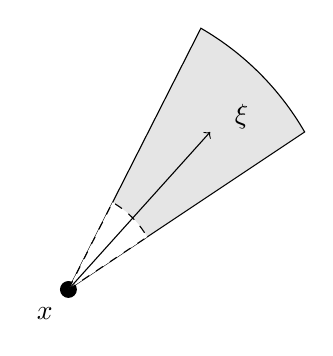
\begin{tikzpicture}
    \draw [fill=black] (0, 0) circle [radius=0.1]; \node at (-0.3, -0.3) {$x$}; 
    
    \filldraw[fill=gray!20!white]
    (0,0) -- (3, 2) arc (30:60:3.6) -- (0,0);
    
    \filldraw[fill=white!20!white, dashed]
    (0,0) -- (1, 0.66666) arc (30:60:1.2) -- (0,0);
    
    \draw [-> ] (0, 0) -- (1.8, 2); \node at (2.2, 2.2) {$\xi$};
    \end{tikzpicture}
    \captionof{figure}{Microlocalisation in phase space. }
\end{center}

\begin{fdefinition}
    The \textbf{wavefront set} of a compactly supported tempered distribution 
    \[
    u \in C^{-\infty}_c(\R^n) = \set{u \in \sch'(\R^n) \wh \supp(u) \Subset \R^n} 
    \]
    is given by 
    \begin{align*}
        \WF(u) = \bigcap \set{\Char^0(A) \wh A \in \Psi^0_\infty(\R^n), Au \in C^\infty(\R^n)}. 
    \end{align*}
    For general tempered distribution $u \in \sch'(\R^n)$, its wavefront set is given by 
    \begin{align*}
        \WF(u) = \bigcup_{\chi \in C^\infty_c(\R^n)} \WF(\chi u). 
    \end{align*}
\end{fdefinition} 

The next proposition shows that wavefront set is a refinement of the singular support. 
\begin{fprop}
    For compactly supported tempered distribution, $u \in C^{-\infty}_c(\R^n)$, 
    \begin{align*}
        \pi(\WF(u)) = \mathrm{singsupp}(u). 
    \end{align*}
    where $\pi(x, y) = x$ is the projection map. 
\end{fprop}
\begin{proof}
    To show $\pi(\WF(u)) \subset \mathrm{singsupp}(u)$, we observe that, by definition of singular support, 
    \begin{align*}
        x_0 \not \in \mathrm{singsupp}(u) \implies \exists \phi \in \sch(\R^n), \, \phi(x_0) \neq 0, \, \phi u \in \sch(\R^n). 
    \end{align*}
    But since multiplication by $\phi$ gives an operator in $\Psi^0_\infty(\R^n)$ which is elliptic at $(x_0, \xi)$ for any $\xi \neq 0$ ($\phi$ is its own principal symbol which happens to be homogeneous and non-zero for any $(x_0, \xi), \xi \neq 0$). Therefore, $x_0 \not \in \pi(\WF(u))$. \\
    \\
    Conversely, if $x_0 \not\in \pi(\WF(u))$, then for all $\xi \neq 0$, there exist $A_\xi \in \Psi^0_\infty(\R^n)$ such that $A_\xi$ is elliptic at $(x_0, \xi)$ and $A_\xi u \in C^\infty(\R^n)$. Since elliptic set $\Ell^0(A_\xi)$ is open and conic, we know that there exist $\epsilon = \epsilon(\xi)$ such that $A_\xi$ is elliptic in the open conic set
    \begin{align*}
        V_\xi = \set{(x', \xi')\in \R^n \times (\R^n \setminus \set{0}) \wh \abs{x' - x_0} < \epsilon, \abs{\widehat{\xi'} - \widehat{\xi}} < \epsilon }. 
    \end{align*}
    Compactness of the sphere (note that $\xi' \mapsto \widehat{\xi'}$ is an embedding of $\R^n \setminus \set{0}$ into $S^n$) allow us to cover $\set{x_0} \times (\R^n \setminus \set{0})$ with finite number of $V_{\xi_j}, j = 1, \dots, N$ with corresponding operators $A_{\xi_j}$. \\
    Now, consider the operator
    \begin{align*}
        A = \sum_{j = 1}^N A^*_{\xi_j}A_{\xi_j}. 
    \end{align*}
    By the pseudolocality of pseudodifferential operators, we know that $A_{\xi_j} u \in C^\infty(\R^n) \implies A^*_{\xi_j} A_{\xi_j} u \in \C^\infty(\R^n)$. Therefore, $Au \in C^\infty(\R^n)$ and $A$ is elliptic at $(x_0, \xi), \forall \xi \neq 0$ with non-negative symbol. We can pick a smooth cut-off $\chi$, $\chi \equiv 1$ when resticted to an $\epsilon/2$-ball around $x_0$ forming an operator
    \begin{align*}
        A + (1 - \chi) \in \Psi^0_\infty(\R^n)
    \end{align*}
    that is globally elliptic. We can construct a (global) elliptic parametrix $E$ so that 
    \begin{align*}
        1 - (E \circ A + E (1 - \chi)) \in \Psi^{-\infty}_\infty(\R^n). 
    \end{align*}
    Finally, we can choose any smooth cut-off $\phi$ with support subordinate to that of $\chi$, i.e. $\supp(\phi) \subset \supp(\chi)$ and note that 
    \begin{align*}
        \phi \circ E \circ (1 - \chi) \in \Psi^{-\infty}_\infty(\R^n)
    \end{align*}
    making it a smoothing operator (by proposition \ref{prop : residual operators are smoothing}). Thus, we conclude 
    \begin{align*}
        \phi u = \phi E \circ A u + \phi \circ E \circ (1 - \chi) u \in C^\infty(\R^n)
    \end{align*}
    as required. 
    
    
    
    
\end{proof}

\subsection{Wavefront set for pseudodifferential operators}
The wavefront set for pseudodifferential operators, or the \textit{essential support} are defined in terms of their symbols. Informally, they are points in phase space, i.e. points $x$ is the base space and a direction $\xi$,  where the symbols have insufficient decay in the $\xi$ direction. 

\begin{fdefinition}
    Let $a \in S^{m}_\infty(\R^{p}; \R^n)$ for some $m \in \R$, $p, n \in \N$ be a symbol. We say $a$ is of order $-\infty$ at a point $(x_0, \xi_0) \in \R^p \times \R^n \setminus \set{0}$ (write $a = O(\sym[\xi]^{-\infty})$) if there exist $\epsilon \in \R_{> 0}$ such that for all $M \in \R$, there is a constant $C_M > 0$ such that 
    \[
    \abs{a(x, \xi)} \leq C_M \sym[\xi]^{-M}
    \]
    in the neigbourhood of $(x_0, \xi_0)$ given by
    \[
    \overline{U}_{(x_0, \xi_0)} = \set{(x, \xi) \in \R^p \times \R^n \wh \abs{x - x_0} \leq \epsilon, \abs{\widehat{\xi} - \widehat{\xi_0}} \leq \epsilon}. 
    \]
    We define the cone support of the symbol $a$ to be all the points in phase space that where it fails to be $O(\sym[\xi]^{-\infty})$. 
    \[
    \mathrm{conesupp}(a) = \set{(x, \xi) \in \R^p \times \R^n \setminus \set{0} \wh a = O(\sym[\xi]^{-\infty}) \text{ at } (x, \xi)}^c. 
    \]
\end{fdefinition}


\begin{flemma}
    Let $a \in S^{\infty}_\infty(\R^{p}; \R^n)$, then 
    \begin{enumerate}
        \item $\mathrm{conesupp}(a)$ is a closed conic set in $\R^p \times \R^n$. 
        \item If $a = O(\sym[\xi]^{-\infty})$ at $(x_0, \xi_0) \in \R^p \times \R^n \setminus \set{0}$, then so is $D^\alpha_x D^\beta_\xi a(x, \xi)$ for any multi-index $\alpha, \beta$
    \end{enumerate}
\end{flemma}
\begin{proof}
    See \cite[Chapter 4]{rbm_intro_microlocal}.
\end{proof}

With the lemma above, we can in fact define the cone support of a symbol to be the smallest closed conic subset of the phase space (with $\xi \neq 0$) such that, in the complement, $a$ and all its derivatives are of order $-\infty$.\\



\begin{fdefinition}
    Let $A \in \Psi^m_\infty(\R^n)$,  $m \in \R$ be pseudodifferential operator. We define the \textbf{essential support}, $\WF'(A)$, of $A$ to be the cone support of its left symbol, i.e. 
    \begin{align*}
        \WF'(A) = \mathrm{conesupp}(\sigma_L(A)) \subset \R^n \times \R^n \setminus \set{0}. 
    \end{align*}
\end{fdefinition}
\hfill \\

\begin{flemma}
    Let $A \in \Psi^m_\infty(\R^n)$, $B \in \Psi^{m'}_\infty(\R^n)$ be pseudifferential operators. Then 
    \begin{enumerate}
        \item $\WF'(A) = \mathrm{conesupp}(\sigma_R(A))$. 
        \item $\WF'(A\circ B) \subset \WF'(A) \cap \WF'(B)$. 
        \item $\WF'(A + B) = \WF'(A) \cup \WF'(B)$. 
    \end{enumerate}
\end{flemma}
\begin{proof}
    See \cite[Section 3]{Vasy2015-oo}
\end{proof}

With the notion of operator wavefront set  we can define the notion of \emph{microlocal elliptic parametrix} which can be thought of as local inverse at an elliptic point of the pseudodifferential operator. 
\begin{fprop}
    Let $A \in \Psi^m_\infty(\R^n)$ and $z \not \in \Char^m(A)$. Then there exist a (two-sided) microlocal parametrix $B \in \Psi^{-m}(\R^n)$ such that 
    \begin{align*}
        z \not \in \WF'(1 - AB) \text{   and   } z \not \in \WF'(1 - BA). 
    \end{align*}
    
\end{fprop}
\begin{proof}
    Let $A \in \Psi^m_\infty(\R^n)$ is elliptic at $(x_0, \xi_0) \in \Ell^m(A)$. For each $\epsilon \in \R_{> 0}$ we define
    \begin{align*}
        \gamma_\epsilon(x, \xi) = \chi\brac{\frac{x - x_0}{\epsilon}} (1 - \chi(\epsilon \xi)) \chi\brac{\frac{\widehat{\xi} - \widehat{\xi_0}}{\epsilon}}
    \end{align*}
    where $\chi \in C^\infty(\R^n)$ is a smooth cut-off function that is identically $1/2$-ball but supported only in the unit ball. Notice that $\gamma_\epsilon \in S^{0}_\infty(\R^{2n}; \R^n)$ with support given by 
    \[
    \supp(\gamma_\epsilon) \subset \set{(x, \xi) \wh \abs{x - x_0} \leq \epsilon,\, \abs{\xi} \geq\frac{1}{2 \epsilon},\, \abs{\widehat{\xi} - \widehat{\xi_0}} \leq \epsilon }. 
    \]
    Restricted to the conic set
    \[
    \overline{U}_{\epsilon} = \set{(x, \xi) \wh \abs{x - x_0} \leq \frac{\epsilon}{2}, \, \abs{\widehat{\xi} - \widehat{\xi_0}} \leq \frac{\epsilon}{2}, \, \abs{\xi} \geq \frac{1}{\epsilon}} \subset \supp(\gamma_\epsilon)
    \]
    it is identically $1$ and therefore $\gamma_\epsilon$ is elliptic at $(x_0, \xi_0)$. Let $L_\epsilon = \mathrm{Op}_L(\gamma_\epsilon)$ be the corresponding pseudodifferential operator. Observe that, by construction 
    \[
    (x_0, \xi_0) \not\in \WF'(1 - L_\epsilon)
    \]
    since $1 - \gamma_\epsilon$ is supported away from an $\epsilon$-neighbourhood of $x = x_0$ and the wavefront set of $L_\epsilon$ is contained in an $\epsilon$-neighbourhood of $(x_0, \xi_0)$, i.e. 
    \[
    \WF'(L_\epsilon) \subset N_\epsilon(x_0, \xi_0) := \set{(x, \xi) \wh \abs{x - x_0} \leq \epsilon, \, \abs{\widehat{\xi} - \widehat{\xi_0}} \leq \epsilon }
    \]
    since $\gamma_\epsilon$ is bounded below in some conic neighbourhood of every point in $N_\epsilon(x_0, \xi_0)$. \\
    \\
    Now, let $G_s = \mathrm{Op}_L(\sym[\xi]^s)$ for each $s \in \R$. Note that $G_s$ is globally elliptic with positive principal symbol. Consider the following operator, 
    \begin{align*}
        J = (1 - L_\epsilon) \circ G_{2m} + A^* A \in \Psi^{2m}_\infty(\R^n)
    \end{align*}
    with principal symbol 
    \[
    \sigma_{2m}(J) = (1 - \gamma_\epsilon)\sym[\xi]^{2m} + \abs{\sigma_m(A)}^2. 
    \]
    Since $\Ell^m(A)$ is open conic, we can choose $\epsilon$ is small enough so that $\Ell^{m}(A) \subset \supp(\gamma_\epsilon)$. Then, by positivity of all terms involved, we have
    \begin{align*}
        \frac{\abs{\sigma_{2m}(J)} }{\sym[\xi]^{2m}}
        &= (1 - \gamma_\epsilon) + \frac{\abs{\sigma_m(A)}^2}{\sym[\xi]^{2m}}
    \end{align*}
    where the first term is bounded below by $1$ outside of $\supp(\gamma_\epsilon)$ while in $\supp(\gamma_\epsilon)$ the second term is bounded below by $\epsilon$ since $A$ is elliptic (of order $m$) at every point in $\supp(\gamma_\epsilon)$. Therefore $J$ is globally elliptic and thus have a global elliptic parametrix $H \in \Psi^{-2m}_\infty(\R^n)$. We shall claim that 
    \[
    B = H \circ A^* \in \Psi^m_\infty(\R^n)
    \]
    is a (right) microlocal elliptic parametrix to $A$. Indeed, 
    \begin{align*}
        B \circ A - 1 
        &= H A^*A - 1 \\
        &= H\brac{J - (1 - L_\epsilon)G_{2m}} - 1\\
        &= (HJ - 1) - H(1 - L_\epsilon)G_{2m}. 
    \end{align*}
    Since $H$ is a global parametrix to $J$, the first term above is a smoothing operator (i.e. an element of $\Psi^{-\infty}_\infty(\R^n)$ and therefore have empty wavefront set. Furthermore, by \cite{wavefront of compositiion} the wavefront set of the second term is a subste of $\WF'(1 - L_\epsilon)$ which does not contain $(x_0, \xi_0)$ by construction. 
\end{proof}


\begin{fcor} \label{cor : microlocal elliptic estimate}
    Let $A \in \Psi^{m}_{\infty}(\R^n)$ and $u \in \sch'(\R^n)$. If for some $Q' \in \Psi^{0}_{\infty}(\R^n)$, $Q'Au \in H^{s}(\R^n)$, then for any other $Q \in \Psi^{0}_{\infty}(\R^n)$ such that $\WF'(Q) \subset \Ell^m(A) \cap \Ell^0(Q')$ we have $Qu \in H^{s + m}(\R^n)$ and it satisfies the estimate: $\forall N \in \R$, $\exists C > 0$ 
    \begin{align*}
    \norm[Qu]_{H^{s +m}} \leq C \brac{\norm[Q'Au]_{H^s} + \norm[u]_{H^N}}. 
    \end{align*}
\end{fcor}
\begin{proof}
    At any point $\alpha \in \WF'(Q)$, $Q'A$ is microlocally elliptic, since $\Ell^2(Q'A) = \Ell^2(A) \cap \Ell^0(Q')$. Therefore, we can construct a microlocal elliptic parametrix $B$ for $Q'A$ near $\alpha$ so that if  $E = BQ'A - 1$ denotes the residue, we have 
    \begin{align*}
    \WF'(QE) = \WF'(E) \cap \WF'(Q) = \emptyset 
    \end{align*}
    This shows that $QE \in \Psi^{-\infty}_{\infty}(\R^n)$. Also, by definition of $E$, 
    \begin{align*}
    Qu = Q (BQ'A - E) u = QBQ'A u - QEu 
    \end{align*}
    where we know that $QB \in \Psi^{-m}_{\infty}(\R^n)$. Using the Sobolev boundedness of the operators
    \begin{align*}
    QB : H^{s + m} \to H^{s}\\
    E : H^{s + m} \to H^N
    \end{align*}
    we get
    \begin{align*}
    \norm[Qu]_{H^{s + m}} \leq \norm[QBQ'Au]_{H^{s + m}} + \norm[QEu]_{H^{s + m}} \leq C \brac{\norm[Q'Au]_{H^s} + \norm[u]_{H^N}}
    \end{align*}
    for some $C > 0$. 
    
\end{proof}

\subsection{Pseudodifferential operators and microlocal}
Just as wavefront set refine the notion of singular support, we have the refinement of the property of pseudolocality of pseudodifferential operator. We refer to \cite{Vasy2015-oo} or \cite{rbm_intro_microlocal} for proof. 

\begin{fprop}
    Pseudodifferential operators are microlocal in the following sense: 
    Let $A \in \Psi^m_\infty(\R^n)$ and $u \in C^{-\infty}_c(\R^n)$, then 
    \begin{align}
        \WF(Au) \subset \WF(u). 
    \end{align}
    In fact, we have 
    \begin{align*}
        \WF(Au) \subset \WF'(A) \cap \WF(u). 
    \end{align*}
\end{fprop}


A partial converse to the above is given by the following proposition. \\

\begin{fprop}
    Let $A \in \Psi^m_\infty(\R^n)$ and $u \in C^{- \infty}_c(\R^n)$, then 
    \begin{align*}
        \WF(u) \subset \WF(Au) \cup \Char^m(A).
    \end{align*}
\end{fprop}

\end{document}